\chapter{Methodology} \label{chap:methodology}
This chapter lays out the methodical steps I took while implementing the project.
Main steps for implementing this project fall into four general categories.
These four categories are:
\begin{itemize}
    \item Establishing a baseline benchmark
    \item Improving metrics beyond baseline benchmark
    \item Ensuring model interpretability is maintained
    \item Deploying the final model to production
\end{itemize}

Further sections will provide detail for these four main categories.

\section{Establishing a benchmark}
The first step to every machine learning project is that model produced is to perform better than any random or naive solution.
Although random guess in any binary classification suggests that the minimum accuracy should be greater or equal than 50\%, because of the imbalance in the test dataset actually requires higher accuracy for this project.
Mainly because we have 390 pneumonia images in the 624 total images in the test dataset dummy classifier that predict pneumonia for any given image will achieve 62.5\% accuracy.
However, given the imbalance of the test dataset accuracy would not be the choice of a good metric for assessing the performance.
For that reason on any experiment conducted, collecting precision, recall as well as calculating f1 score will be utilized.
If I introduce these metrics in more detail.
Precision is calculated by dividing true positives (tp) in predictions to true positives and false positives (fp).
\begin{equation}
    Precision = \frac{tp}{tp + fp}
\end{equation}

The recall is calculated by dividing true positives to true positives and false negatives (fn).

\begin{equation}
    Recall = \frac{tp}{tp + fn}
\end{equation}

To capture the correct performance of the classifier we need to consider both precision and recall.
F1 score provides the ability to consider both precision and recall for the same classification problem because it is calculated by getting a harmonic mean of the precision and recall.

\begin{equation}
    F_1 = \frac{2}{\frac{1}{precision} + \frac{1}{recall}} = 2 \times \frac{precision \times recall}{precision + recall}
\end{equation}


Next part for the benchmarking is choosing which algorithms to train on the data for benchmarking.
Given we don't know the distribution of the data, training fundamental machine learning algorithms together with the neural network algorithms is a cautious step to take. 
For that reason, I have chosen to train two fundamental machine learning algorithm, namely the Random Forest classifier and the Support vector classifier as a part of establishing a benchmark.


\subsection{Random Forest Classifier}
For the past years, tree-based algorithms have been very popular in the academic community as well as in the industry with numerous papers demonstrated in ICML, NIPS and JMLR.
Random forest emerges in this category as a very strong algorithm by Breiman~\cite{randomforest} that achieves remarkable performance in small to a medium dataset.
The final baseline will be determined by finding an optimal number of estimators and maximum features using cross-validation.


\subsection{SVM Classifier}
In addition to Random Forest, the secondary mainstream machine learning algorithm is Support Victor Machine classifier~\cite{svm}.
The biggest factor for choosing this algorithm was its robustness in detecting non-linear features in the data using kernel trick.
Similarly to Random Forest hyper-parameters chosen with cross-validation.

\subsection{LeNet-5}
LeNet-5~\cite{Lenet5} is the first one of the well-known CNNs that I will apply to this problem to consider in baseline benchmark.
I kept the attributes of the network as close to the origin network as possible but some characteristic of the network had to be changed when it is trained on this classification problem.
The first difference in this project needed in input and output layers, MNIST dataset have ten classes therefore required ten dense neurons at the output layer in the original network but in this project, there are two classes to predict which can be achieved by having one dense output neuron instead.
Input layer also changed because $32 \times 32$ is not a suitable resolution for the pneumonia detection and changed to $224 \times 224$ for better representation.
Another change made to this model is using relu activation function rather than hyperbolic tangent function (tanh) because of the less than ideal gradient flow in saturated tanh function prevented model to converge to a good solution.
Detail of the model summary given below for reference.

\begin{verbatim}
    Model: "LeNet-5"
_________________________________________________________________
Layer (type)                 Output Shape              Param #   
=================================================================
conv2d_6 (Conv2D)            (None, 220, 220, 6)       456       
_________________________________________________________________
average_pooling2d_4 (Average (None, 110, 110, 6)       0         
_________________________________________________________________
conv2d_7 (Conv2D)            (None, 106, 106, 16)      2416      
_________________________________________________________________
average_pooling2d_5 (Average (None, 53, 53, 16)        0         
_________________________________________________________________
conv2d_8 (Conv2D)            (None, 49, 49, 120)       48120     
_________________________________________________________________
flatten_2 (Flatten)          (None, 288120)            0         
_________________________________________________________________
dense_6 (Dense)              (None, 120)               34574520  
_________________________________________________________________
dense_7 (Dense)              (None, 84)                10164     
_________________________________________________________________
dense_8 (Dense)              (None, 1)                 85        
=================================================================
Total params: 34,635,761
Trainable params: 34,635,761
Non-trainable params: 0
_________________________________________________________________
\end{verbatim}

\subsection{AlexNet}
Similar to LeNet-5, AlexNet~\cite{Alexnet} also aimed to the kept original structure as much as possible.
AlexNet comprises of eight layers, five of those were convolution layers where some of them connected to max-pooling layer. 
Despite the fact, the architect is preserved almost same as the original implementation additional steps such as adding local response normalization or PCA augmentation is not applied because of the ad hoc nature of the process and limited effect of this processes in the final performance.
AlexNet is ultimately a very influential paper that steers the direction for how the CNNs are designed and fueled the adoption of the use of neural networks in many fields.
Fallowing quote from the paper also explains the reason why neural networks gain so much popularity and pushing the state of the art results year after year.
\begin{quote}
    \textit{"All of our experiments suggest that our results
can be improved simply by waiting for faster GPUs and bigger datasets to become available."}
\end{quote}

\begin{verbatim}
    Model: "AlexNet"
_________________________________________________________________
Layer (type)                 Output Shape              Param #   
=================================================================
conv2d_10 (Conv2D)           (None, 54, 54, 96)        34944     
_________________________________________________________________
max_pooling2d_6 (MaxPooling2 (None, 26, 26, 96)        0         
_________________________________________________________________
conv2d_11 (Conv2D)           (None, 26, 26, 256)       614656    
_________________________________________________________________
max_pooling2d_7 (MaxPooling2 (None, 12, 12, 256)       0         
_________________________________________________________________
conv2d_12 (Conv2D)           (None, 12, 12, 384)       885120    
_________________________________________________________________
conv2d_13 (Conv2D)           (None, 12, 12, 384)       1327488   
_________________________________________________________________
conv2d_14 (Conv2D)           (None, 12, 12, 256)       884992    
_________________________________________________________________
max_pooling2d_8 (MaxPooling2 (None, 5, 5, 256)         0         
_________________________________________________________________
flatten_2 (Flatten)          (None, 6400)              0         
_________________________________________________________________
dense_6 (Dense)              (None, 4096)              26218496  
_________________________________________________________________
dropout_4 (Dropout)          (None, 4096)              0         
_________________________________________________________________
dense_7 (Dense)              (None, 4096)              16781312  
_________________________________________________________________
dropout_5 (Dropout)          (None, 4096)              0         
_________________________________________________________________
dense_8 (Dense)              (None, 1)                 4097      
=================================================================
Total params: 46,751,105
Trainable params: 46,751,105
Non-trainable params: 0
_________________________________________________________________
\end{verbatim}

\subsection{VGGNet}
VGGNet is one of the best performant in 2014 ILSVRC competition that get a best performance in classification and localization task.
There are two different variation of this network is available namely the VGGNet 19 and VGGNet 16. 
For this project 16 layered VGGNet 16 is a good choice it has a sufficient capacity given that the dataset is relatively small.
Main contribution of the VGGNet is that it demonstrated the importance of the network depth to good performance.
Layer structure of the architecture is straightforward, only performs $3 \times 3$ convolution with $2 \times 2$ pooling.
Similarly, for the purpose of the benchmarking architecture kept as close to original as possible with only change is made to final layer replaced with one neuron dense layer to accommodate the binary classification task.
Advantage of using this network is that it is implemented in most of the modern software packages and it also available to initialize with the weights of imagenet. 
That property will be very useful for comparing the performance when transfer learning is explored in subsection \ref{subsec:transferlearning}.
Detail of full network listed below.

\begin{verbatim}
    Model: "VGGNet"
_________________________________________________________________
Layer (type)                 Output Shape              Param #   
=================================================================
input_4 (InputLayer)         [(None, 224, 224, 3)]     0         
_________________________________________________________________
vgg16 (Functional)           (None, 512)               14714688  
_________________________________________________________________
dense_3 (Dense)              (None, 4096)              2101248   
_________________________________________________________________
dropout_2 (Dropout)          (None, 4096)              0         
_________________________________________________________________
dense_4 (Dense)              (None, 4096)              16781312  
_________________________________________________________________
dropout_3 (Dropout)          (None, 4096)              0         
_________________________________________________________________
dense_5 (Dense)              (None, 1)                 4097      
=================================================================
Total params: 33,601,345
Trainable params: 33,601,345
Non-trainable params: 0

\end{verbatim}

% \subsection{ResNet}

\section{Improving Performance}
After establishing a benchmark for minimum acceptable performance, this step of will focus on continuously improving the performance on the problem. 
Materialize that goal I have chosen two method, applying transfer learning and building custom neural.

\subsection{Transfer Learning} \label{subsec:transferlearning}
Transfer learning is fundamentally taking weights (or features) learned on one problem, and applying them to similar or new problem that could benefit from it.
Transfer learning usually considered when the training data is too small to train a deep neural network from a scratch.
Process for transfer learning is simple, architecture that will be use in problem in hand is initialized with the weights learned from another problem without the top part of the model.
Here top part is refers to the layer(s) at the end of the model which has got the high level of the features specific to the problem.
And given that the lower layers of the model contribute to simply features like vertical and horizontal lines or edges, weights in these layers held frozen to allow feature extraction from the images in new problem.
After that step top part of the model initialized with the random weight to be trained on the new dataset to learn higher level features.
Transfer learning sometimes get adopted with the concept of \emph{fine-tuning}, which is a process of unfreezing the part of it or the entire model and re-training it with the new data.

Because the dataset of this project is suffering from a small data problem, transfer learning is utilized to discover if generic datasets like imagenet~\cite{imagenet} can be helpful to improve existing model.
Effectiveness of the transfer learning will be measured by training the VGG16 network with the imagenet weights and comparing the performance against same network with randomly initialized version from the benchmarking experiments.

\subsection{Custom Model Architecture}
Another method available to get higher performance in machine learning is to designing custom architect better reflect the data representation.
Despite the great potential of better performance, this method is usually more complex in nature because of the challenges in hyper-parameter search.
Modern CNNs have significantly more hyper-parameters compare to traditional machine learning algorithms. 
For instance, below items are non-exhaustive list of hyper-parameters to consider when designing custom architecture.

\begin{itemize}
    \item Learning rate $\alpha$
    \item Momentum term $\beta$
    \item Number of layers
    \item Number of units in a layer
    \item Kernel size for convolution layers
    \item Type of the convolution layer
    \item Learning rate decay
    \item Type of optimization algorithm
    \item Regularization type and quantity
    \item Mini batch size
\end{itemize}

Complexity of the task gets significantly higher when the attributes such as convolution layers padding and strides included in the number of layer and kernel size.
When used with valid padding convolutional layer have addition constrain that the further layers have to be compatible with the output tensor shapes from previous layers.
Given these complexities and limited time frame of this project some aspects of the hyper-parameter search will be determinant.
Grid search and random search are two of the widely used method when determining the right hyper-parameters.
Studies suggests that random search is more efficient and computationally inexpensive than the grid search in the context of neural network~\cite{randomsearch}.

\begin{figure}[H]
    \centering
    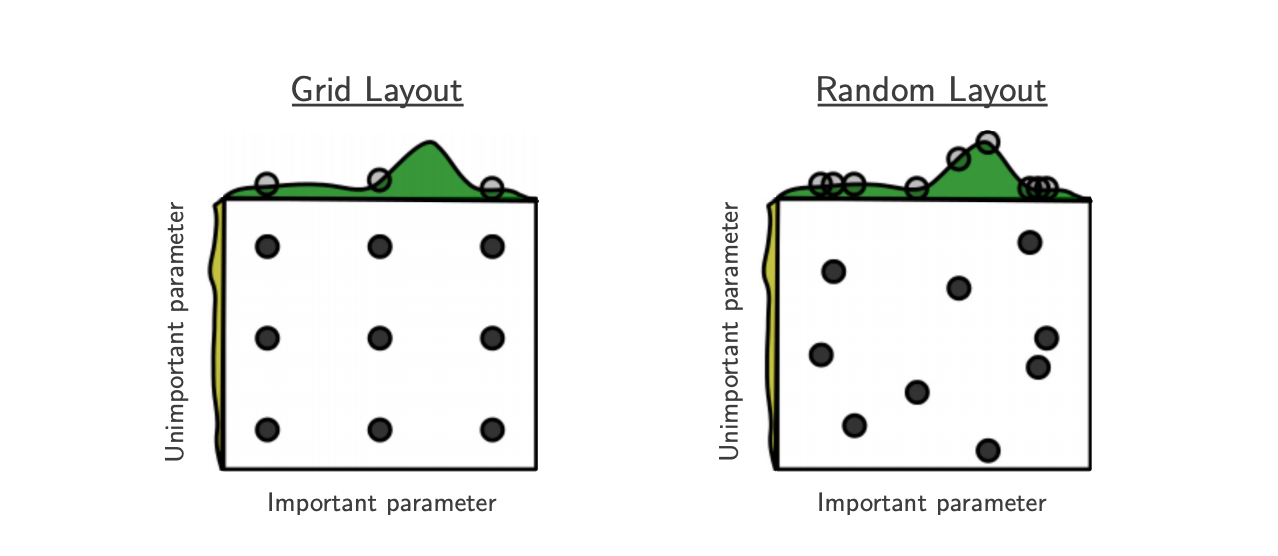
\includegraphics[width=\textwidth]{img/randomsearch.png}
    \caption{Random search versus grid search~\cite{randomsearch}}
    \label{fig:randomsearch}
\end{figure}

For the custom architecture I will be running experiments with random search over the fallowing hyper-parameters.

\begin{itemize}
    \item Type of convolutional layer. Conv2D versus Depthwise convolution
    \item Number of layers
    \item Different convolution blocks (e.g. Inception, residual, etc.)
    \item Type of regularization (e.g. Batch normalization, Dropout)
\end{itemize}

\section{Model Interpretability}
Machine learning models and more specifically neural network usually regarded as black box machines.
Meaning that reason for their predictions are unknown.
However there are variety of techniques that design to elaborate the machine learning models emphasis points.
Before any model put into production it should also be examined for their predictive reasons and because of that I added model interpretability rules before making decision to promote any model to deployment stage.
One such technique call GradCAM~\cite{heatmap} is designed to highlight the areas in the image that contributes the most for the prediction machine learning outputs.

\subsection{GradCAM}
GradCAM~\cite{heatmap} is part of the general visualization technique called \emph{class activation map} (CAM).
It consist of creating a heatmap of activations over the input image space.
A class activation heatmap is a two dimensional surface of scores for individual class mapped in to the corresponding location. For instance, if the input image is with pneumonia heatmap is indicates the areas that most represent pneumonia like features found and vice versa for images that absent of pneumonia.
This technique originally designed for softmax output with different classes and to adapt it to binary classification with sigmoid output, additional logic based on assigning classification with probability grater that 0.5 to pneumonia presence and absence of it to those less that 0.5 probability.

\section{Deployments with CI/CD}
Upon discovery of best performer model up to this point, if the model satisfies the interpretation stage, can added to model folders as a candidate for production release.
Please note that due to manual nature of the model interpretation stage this project utilize continuous development rather than continuous deployment.
Because even though visualization for GradCAM can be generated in an automated fashion there is no measurable criteria available to asses that step.
After the insertion of the model to model folder test suite for the project will run and if the tests are successful, deployment script will automatically run to produce the model artificial needed for the deployment.
Final step in this process is to commit the most recent artifact to central code repository for deployment.
This process repeats ever time when there is a better performer model found.
Detailed information about the deployment choice and the assessment of the deployment is covered in chapter \ref{chap:deployment}.
